\begin{wrapfigure}{r}{4.2cm}
  \centering
  \vspace{-.95cm}
  \begin{tikzpicture}
    \node (s) at (0,0) {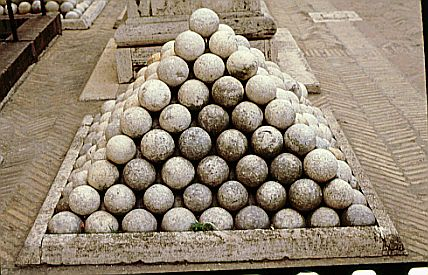
\includegraphics[width=4cm]{images/cannonballs.jpg}};
    \node at (s.south) {\raisebox{-2ex}{\scriptsize (http://tinyurl.com/3bxx2t)}};
  \end{tikzpicture}
  \vspace{-1.0cm}
  \caption{The face centered cubic packing}
  \vspace{-1.0cm}
\end{wrapfigure}
%% alternative images are
%% http://cosmicadventure.com/gallery/albums/album48/Cannonballs_2.jpg
%% http://mathworld.wolfram.com/images/eps-gif/CircleSpherePacking_800.gif
%% http://en.wikipedia.org/wiki/Image:Close-packed_spheres.jpg

\begin{background}
The target of our case study is the Flyspeck Project, which seeks to formally
verify Thomas Hales' proof of the Kepler
Conjecture~\cite{Hales:2005:Annals,Hales:2006:DCG}.  This conjecture asserts
that the density of a packing of unit spheres in 3 dimensions is at most
$\pi/(3\sqrt{2})$, the density of the face centered cubic and hexagonal close
packings.  Posed by Kepler in 1611, it formed part of Hilbert's
18\textsuperscript{th} problem, and until its solution was recognized as one of
the most famous unsolved problems of mathematics.  Hales' proof, completed in
1995, was not accepted immediately by the mathematical community.  Besides its
considerable length, the proof relies essentially on computer calculations.  The
300 pages of text and many thousands of lines of computer code made checking the
proof for errors in the referee process unusually difficult, leading to a
publication delay of nearly 10 years.  In 2003, Hales proposed using computers
to rigorously check the entire proof in detail, including the computer code.  He
dubbed this effort \textit{Flyspeck}\footnote{The word ``flyspeck'' means, ``to
  examine closely''.  It was found by Hales using a regular expression search of
  an English dictionary for the expression ``F.*P.*K'', for ``Formal Proof of
  Kepler''}.  The software systems used in such formalizations are called
\textit{theorem provers} or \textit{proof assistants}\footnote{The word
  ``formalize'' is used in many contexts in this field.  In the remainder of
  this paper, we use ``formal'' and ``formalize'' loosely, possibly referring to
  any degree of colloquial or scientific formalization.  We use ``computerized''
  to mean that a theorem, proof or definition has been expressed in a proof
  assistant.  Note that we consider computerized definitions and proofs formal
  ``documents'' as well.}, examples being Isabelle~\cite{Paulson:1994:Isabelle},
Coq~\cite{Bertot:2004:CoqBook}, and Twelf~\cite{Schurmann:1999:Twelf}.  With
adequate human assistance they can verify that a purported proof follows from a
given set of axioms and inference rules.

Modern proof assistants are still far from being able to check proofs at the
level given in most journals and textbooks.  A typical estimate is that it takes
about a week to formalize a single page of mathematical text.  Hales expects
that it will take around 20 man-years to complete Flyspeck.  Hales is compiling
a {\LaTeX} book~\cite{Hales:2008:FlyspeckBook} of lemmas from different areas of
mathematics that are needed in his proof.  Its 450 pages contain a significant
percentage of the mathematical results used in the proof, covering such
disparate topics as plane, solid, and spherical geometry, graph theory and
hypermaps, single and multivariable calculus, and plane and spherical
trigonometry.

The first steps toward a computerized proof have already been taken.  Nipkow and
Bauer~\cite{Nipkow:2005:Tame} proved the correctness of a fundamental algorithm
in Isabelle.  The other two main parts of the computer code, linear programming
and global optimization, are currently being investigated in doctoral
dissertations~\cite{Zumkeller:2006:TaylorModels,Obua:2005:LinearPrograms}.  A
project page documents some of this progress and has a source repository
containing the book of lemmas, as well as the formalized definitions of some
important functions and inequalities~\cite{website:FlyspeckProjectPage}.
Despite this considerable progress on the computer code, the bulk of the
mathematical formalization remains to be done.  This formalization will consist
of two broad phases.  First, a number of elementary mathematical theories
(e.g. spherical geometry) need to be defined and the relevant lemmas proved.
Then the specific aspects of the Kepler proof that relies on the elementary
results need to be formalized.  Given the content of the book mentioned above,
we suspect that Flyspeck, in its final form, will consist of dozens of theories,
with hundreds of definitions and thousands of lemmas.
\end{background}

\begin{motivation}
\claim{Flyspeck is particularly appealing as a use case for a semantic wiki
approach.}  While the ultimate result is to be a highly formal computerized proof,
the current proof involves both highly formal and semi-formal mathematical
knowledge.  It contains descriptive and motivating yet informal text that should
be preserved for human understanding.  This quasi-formal information would be
difficult to present in a strictly formal setting of a proof assistant.
Secondly, the large number of lemmas, many independent or only loosely coupled,
suggests a ``crowdsourcing'' approach will be beneficial. \claim{Both can be supported
by a (semantic) wiki, as we will show in the following.}
\end{motivation}

%%% Local Variables: 
%%% mode: latex
%%% TeX-master: "flyspeck-wiki-eswc08"
%%% End: 
